\chapter{Evaluation}
In this chapter, I provide a overview of the methods and tests
conducted in the context of my research. The primary focus involves a
comparative analysis of the two introduced designs through various
microbenchmarks. The overarching objective is not solely to contrast these two
designs but to establish a threshold for the activation time of the Control
Core. Additionally, I aim to determine the point at which a transition to a
different core becomes beneficial in terms of the quantity of saved registers
that do not require preservation on the Control Core.

\section{Benchmarks}
For the benchmarks employed in this study, I devised two distinct
scenarios to facilitate the testing process. The first benchmark involves a
straightforward system call-like entry into the Mode Switch Mode, followed by a
return to the original mode. In this case, since there is no transition to
another mode, only three temporary registers are preserved to provide the Mode
Switch Mode with some registers to utilize. It's worth noting that on the
Control Core, such preservation is unnecessary due to its inherent structure,
which includes dedicated registers for its operations. The primary objective of
this particular test is to identify a threshold at which the transition to a
second CPU becomes too expensive. Therefore this benchmark is run with a variety
of delay timings for Control Core activation. To simulate both directions
of the activation process, this delay is incorporated during the activation of
both the Control Core and the main CPU. It is given in the time that one
instruction takes to be executed. So a delay of one means that the activation of
the other core takes the time that one instruction would take to execute. The
general control flow of this benchmark is illustrated in Figure
\ref{fig:syscall}.\par

\begin{figure}[h]
    \centering
    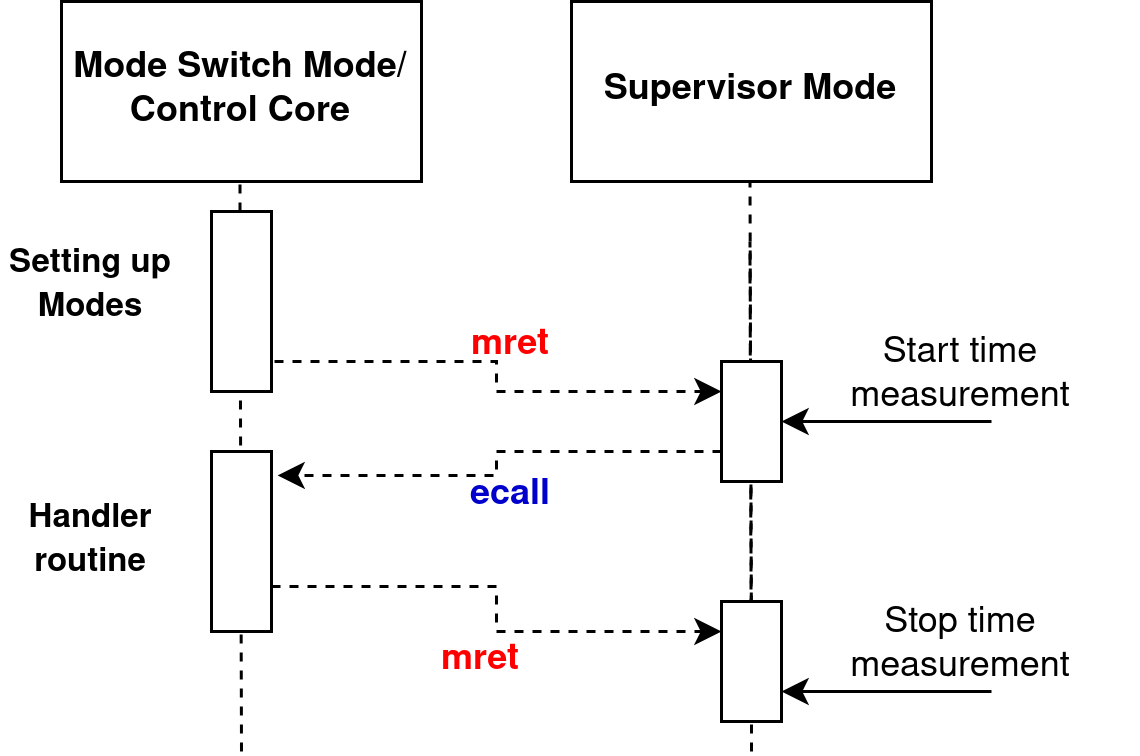
\includegraphics[width=0.5\textwidth]{syscall}
    \captionsetup{justification=centering}
    \caption{Control Flow for simple call into the Mode Switch Mode}
            The control flow changes that happen during a call from the
            supervisor mode (the start mode) into the Mode Switch Mode and back.
            Red depicts instruction executed by the Mode Switch Mode or Control
            Core, blue instruction executed by the other modes. The start and
            end of the timing measurements before and after the \texttt{ecall}
            in the supervisor mode is marked. 
    \label{fig:syscall}
\end{figure}

The second benchmark emulates a comprehensive mode switch from one mode to
another. As depicted in Figure \ref{fig:modeswitch}, the original mode is exited, and the Mode
Switch Mode or Control Core assumes control of the mode-switching process.
Subsequently, the new mode is entered, quickly transitioning back into the Mode
Switch Mode or Control Core, which then transfers control back to the initial
mode. The objective of this benchmark is to identify a threshold of
registers that should be preserved, determining the point at which it becomes
advantageous to switch to a different CPU that doesn't necessitate such
preservation. To ascertain this threshold, the benchmark is executed with
varying numbers of saved registers.\par

\begin{figure}[h]
    \centering
    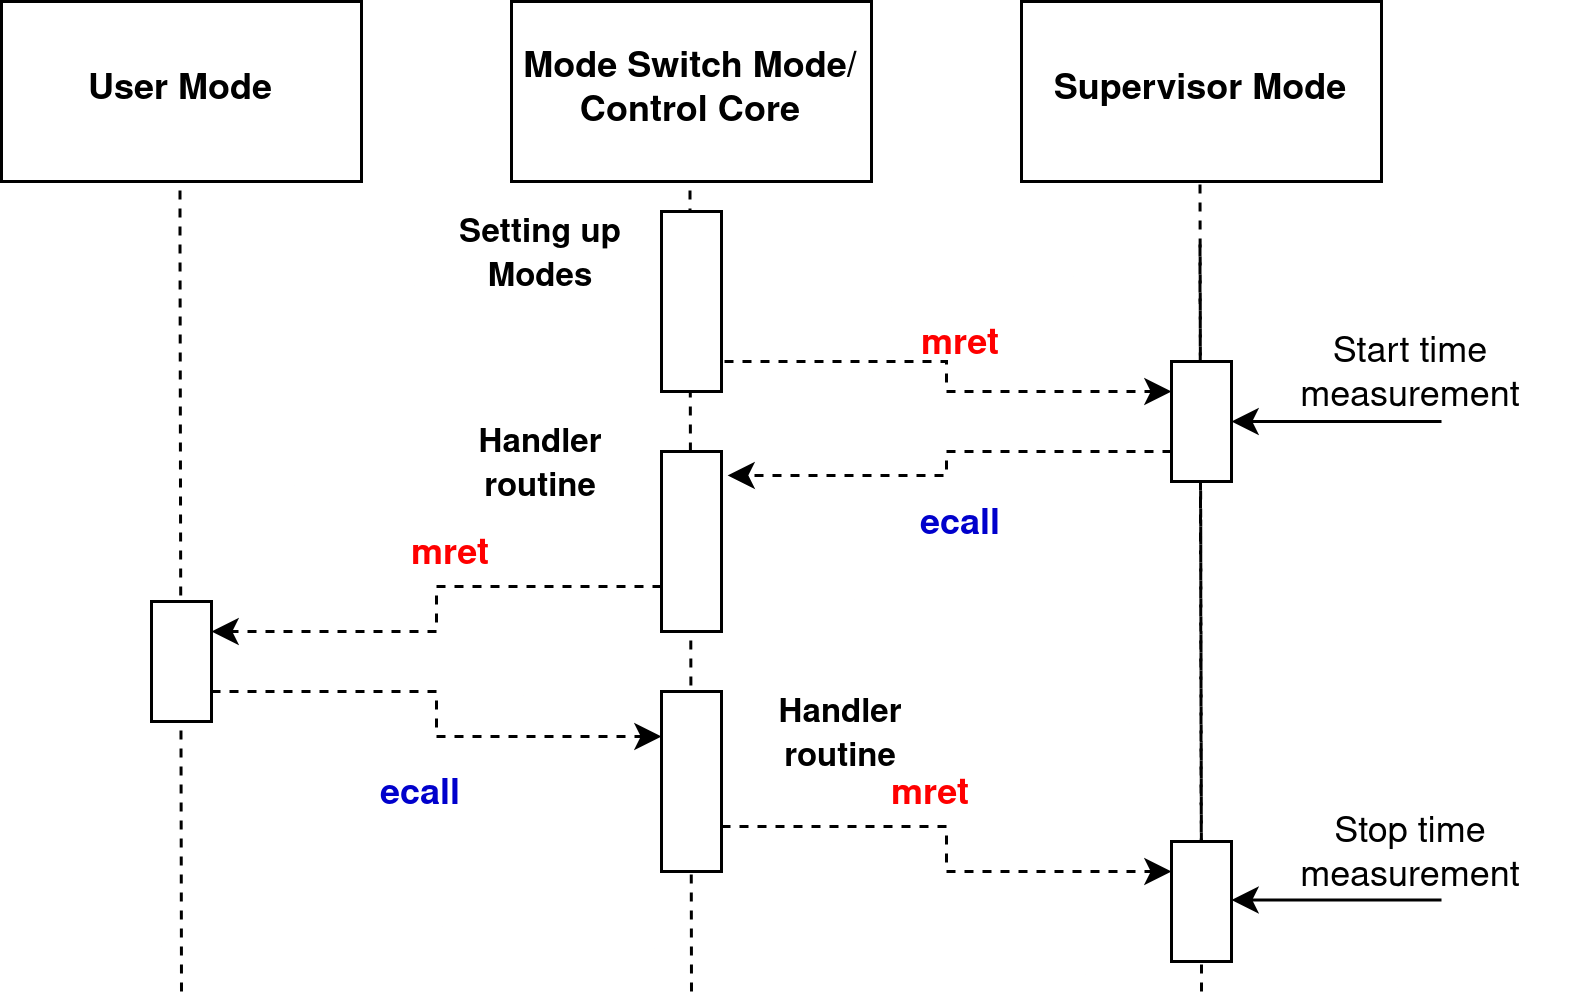
\includegraphics[width=0.8\textwidth]{modeswitch}
    \captionsetup{justification=centering}
    \caption{Control Flow for a mode switch}
            The control flow changes that happen during a transition from the
            supervisor mode (the start mode) to the user mode. Red depicts
            instructions executed by the Mode Switch Mode or Control Core, blue
            instructions executed by the other modes. The start and end of the
            timing measurements before and after the \texttt{ecall} in the supervisor
            mode is marked. 
    \label{fig:modeswitch}
\end{figure}

In both scenarios, the mode switch is initiated through the \texttt{ecall}
instruction from the mode which is left. Therefore the mode switch can be seen
as a ``system call" to the Mode Switch Mode
or Control Core with a request to transition to a specific mode. Notably, this
system call does not include any arguments, as the current routine for mode
switching is hardcoded to either return to the original mode or transition to
the only other mode in the system. It's important to acknowledge that in a real
system, a sophisticated handler would need to make various decisions, a
consideration not addressed in this context. In this benchmarks the overhead for
a minimal handler is investigated. The existing handler simplifies the
process by loading all necessary information from the MLB and returning to the
loaded mode. These modes are established before the start of any
measurements. The measurement period starts just before the \texttt{ecall}
instruction triggers the entry into the Mode Switch Mode or Control Core,
ends right after the original mode is reentered. Consequently, the first
benchmark measures only one entry and one exit to the Mode Switch Mode or
Control Core, effectively quantifying the switch timing. Conversely, the second
benchmark evaluates a complete roundtrip from one mode to another and back,
taking into account the side effects of register saving and restoring between
modes.\par
For a benchmark comparison with an unmodified CPU, the time required for a
mode switch was measured using a methodology similar to that of the
first benchmark. The measurement starts just before an \texttt{ecall} and concludes
upon entry into the trap handler. This models the same case as the benchmarks
for the Modes Switch Mode and Control Core because we leave one mode and end up
in a different one. I will describe this on a short example. Lets say the mode
we are leaving is the user mode. We call \texttt{ecall} which leaves this mode
and end up in the new mode, we will call it the supervisor mode, where the
handler is located. If we start measuring right before the \texttt{ecall} in the
user mode and stop after entering the new mode we measured the overhead of
mode switching. When we start measuring before the \texttt{ecall} and end after
leaving the Mode Switch Mode and Control Core, this measures the overhead of the
mode switching because we also measure what time it takes to come from one mode
in which we can execute to an other mode in which we can execute.\par
The performance evaluation of the MLB is carried out implicitly only when
measuring the switch behavior, involving some loads and stores to the buffer.
However, there is no explicit measurement conducted for the performance of the
PLB. Von Elm\cite{Cve} has previously executed microbenchmarks specifically
addressing the access to these buffers in his work. So I decided to go with his
zero latency buffers for this work.

\section{Setup}
The microbenchmarks were executed using the gem5 simulator, employing a defined
test setup specified through a Python script. The choice was made to utilize the
o3 CPU model in gem5, which emulates an Out-of-Order CPU. This selection was
based on its reputation as the most accurate CPU model offered by gem5. The size
of the PLB and MLB proved less critical for these benchmarks, leading to the
decision to adhere to their standard values of 64 entries. The memory
configuration utilized was a SingleChannelDDR3\char`_1600, with all other parameters
left at their default initialization. Both the system clock and CPU clock were
set to 1GHz.

\section{Results}

\begin{figure}[h]
    \centering
    \includesvg[width=0.8\textwidth]{simple_syscall}
    \captionsetup{justification=centering}
    \caption{Simple syscall into the Mode Switch Mode}
        Comparsion of the Mode Switch Mode performance for 3 saved registers in
        red and the Control Core with a variety of delays in blue. For better
        visibility the  cycles for completion at the y axis start at 250.
    \label{fig:simple_modeswitch}
\end{figure}

Figure \ref{fig:simple_modeswitch} illustrates the cycles required to complete a call into the Mode Switch
Mode and back. The red line shows the cycles that the Mode Switch Mode needs to
do this, the blue bars show the same task for the Control Core with delays from
one instruction to ten instructions for its activation. The data reveals that
activating the Control Core starting at a delay of 6 instructions or more is
slower than entering the Mode Switch Mode on the same CPU and save 3 registers.
Visible by the red line crossing the blue bars beginning at 6 instructions. The
disparity in speed becomes even more pronounced for a complete roundtrip between
modes. Examining Figure \ref{fig:reg_modeswitch}, it becomes evident that even
saving just three registers incurs an overhead nearly twice as much as switching
to a different core with a 1-cycle activation time. As anticipated, the gap
between switching to the Control Core and the Mode Switch Mode widens further as
more registers are saved. This escalation is attributed to the fact that the
Mode Switch Mode not only necessitates saving registers but also restoring them,
resulting in two memory operations for each saved register.
An additional factor contributing to this overhead is the Risc-V's general
approach to register saving. The \texttt{sw} instruction is employed to save a register,
requiring both the register and the address where the register value should be
stored. To prevent the loss of a register during address loading, the \texttt{sscratch}
CSR comes into play as a scratch register, allowing the storage of one register
value to retain a register for storing the address. Once registers are saved,
the value from \texttt{sscratch} can be restored. Consequently, three
instructions are necessary for each register that needs saving: one for saving a
register to the \texttt{sscratch} CSR, one for loading the address, and one for restoring
the register. This entire overhead is avoided when transitioning to a
second CPU. The results of this two benchmarks leads to the conclusion that a
threshold of a delay of 6 instructions to activate the Control Core can be enough to make it more
performant than the Mode Switch Mode.\par

\begin{figure}[h]
    \centering
    \includesvg[width=0.8\textwidth]{reg_modeswitch}
    \captionsetup{justification=centering}
    \caption{Modeswitch with register saving}
        Comparison between Mode Switch Mode and Control Core when switching to
        another mode and back while saving different amounts of registers for
        the Mode Switch Mode, depicted by the lines.
    \label{fig:reg_modeswitch}
\end{figure}

The comparison with a syscall in an unmodified CPU, as illustrated in Figure \ref{fig:unmod_cpu},
reveals that both analyzed implementations introduce a considerable performance
overhead. While this outcome is anticipated, it underscores that the enhanced
flexibility offered by both approaches is accompanied by a substantial
performance cost. Determining the
superior solution for achieving the flexibility of freely definable modes depends
on more factors than just performance, with hardware complexity and cost
emerging as the foremost considerations. The efficiency of the Control Core is
dependent on its tight integration with the CPU, ensuring swift execution of
every change. However, achieving such integration could lead to a highly
complex implementation, particularly if the objective is to emulate a fully
functional CPU. Consequently, a critical question arises concerning the
cost-effectiveness of such a hardware implementation. 
Sustainable hardware production necessitates mass adoption, implying
ease of adoption. To achieve this, it is imperative to minimize software
complexity. In this regard, the Control Core appears to outperform the Mode
Switch Mode. In the latter, programmers must continually be vigilant about which
registers are saved or not, and avoid actions that might unintentionally alter
the CPU state. In contrast, the Control Core maintains a strict separation from
the main CPU, mitigating such concerns. Currently the Control Core seems quite
ineffective when its only purpose is to not access the registers. Some other
designs might be better for this usecase. However, making a conclusive judgment on
which design is more suitable for implementing software-defined CPU modes
requires additional insights into hardware intricacies and the associated
implementation costs.

\begin{figure}[h]
    \centering
    \includesvg[width=0.3\textwidth]{unmod_cpu}
    \captionsetup{justification=centering}
    \caption{Comparsion to an unmodified CPU}
        Comparsion between the two new designs and an unmodified CPU during a
        simple Syscall shows the huge performance overhead.
    \label{fig:unmod_cpu}
\end{figure}


\chapter{Future Work}
The preceding chapters have presented results from the examination of these two
prototypes, showcasing the potential for a more flexible implementation of
modes but also brought up some other challenges. Among these challenges, a paramount
concern is the need for more realistic benchmarks. A comprehensive evaluation
would involve the adaptation of a simple operating system to these prototypes
and the formulation of application benchmarks.\par
Another dimension that demands exploration, achievable only within a more
complex system, involves the development of a specialized library for mode
support. Such a library could potentially alleviate the aforementioned code
complexity associated with the Mode Switch Mode. Addressing these aspects in
future work will contribute to a more comprehensive understanding of the
capabilities and challenges associated with the implementation of flexible CPU
modes.\par
Another crucial aspect to address in future work involves the comparison with
real hardware. As highlighted in the evaluation chapter, a comprehensive
understanding of the designs necessitates insight into the intricacies of the
underlying hardware. Without such knowledge, any comparison between the two
designs remains inherently incomplete. A preliminary step towards closing this
gap could involve conducting a high-level synthesis of the designs to provide an
initial approximation of their feasibility and cost.\par
Furthermore, an alternative design consideration worth exploring is the
integration of special registers into the Mode Switch Mode. While the Mode
Switch Mode grapples with the challenges of saving registers, both in terms of
performance and code complexity, the efficiency and cost-effectiveness of the Control
Core in a real hardware context may pose concerns. Introducing special
registers, akin to the shadow registers employed by ARM, could potentially
address the register-saving problem without incurring the substantial
performance costs associated with a secondary CPU. Investigating these aspects
in real hardware scenarios will contribute valuable insights to the overall
evaluation and refinement of the proposed designs.\par
Upon delving into the intricacies of software-defined mode switches and
optimizing their details, the exploration of additional questions concerning use
cases becomes paramount. Already existing approaches for code splitting on a
compiler level, like the one proposed by Huang et al.\cite{HSB} for android applications,
could be adopted to multiple CPU modes. Understanding the strategic placement of specific code
within specialized modes prompts inquiries into the practical implications of
such configurations. Beyond the inherent safety benefits associated with mode
switches, there arises the question of potential performance benefits derived
from executing specific segments of software within these modes by eliminating
some security bottlenecks like switches to higher privilege levels. Identifying
scenarios where running code in a special mode makes sense and discerning the
performance advantages conferred by such configurations contribute to a more
comprehensive understanding of the practical implications and optimizations
achievable through software-defined CPU modes.